\documentclass[12pt]{article}
\usepackage{geometry}                % See geometry.pdf to learn the layout options. There are lots.
\geometry{letterpaper}                   % ... or a4paper or a5paper or ... 
\usepackage{graphicx}
\usepackage{amssymb}
\usepackage{amsthm}
\usepackage{epstopdf}
\usepackage[utf8]{inputenc}
\usepackage[usenames,dvipsnames]{color}
\usepackage[table]{xcolor}
\usepackage{hyperref}
\DeclareGraphicsRule{.tif}{png}{.png}{`convert #1 `dirname #1`/`basename #1 .tif`.png}

\theoremstyle{definition}
\newtheorem{example}{Example}

\newcommand{\projectname}{Smart Shopping List}
\newcommand{\productname}{Smart Shopping List}
\newcommand{\projectleader}{A. Walliser}
\newcommand{\documentstatus}{In process}
%\newcommand{\documentstatus}{Submitted}
%\newcommand{\documentstatus}{Released}
\newcommand{\version}{V. 1.0}

\begin{document}
\begin{titlepage}
\begin{flushright}

\includegraphics[scale=.5]{htlleondinglogo.png}\\
\end{flushright}

\vspace{10em}

\begin{center}
{\Huge System Specification} \\[3em]
{\LARGE \productname} \\[3em]
\end{center}

\begin{flushleft}
\begin{tabular}{|l|l|}
\hline
Project Name & \projectname \\ \hline
Project Leader & \projectleader \\ \hline
Document state & \documentstatus \\ \hline
Version & \version \\ \hline
\end{tabular}
\end{flushleft}

\end{titlepage}
\section*{Revisions}
\begin{tabular}{|l|l|l|}
\hline
\cellcolor[gray]{0.5}\textcolor{white}{Date} & \cellcolor[gray]{0.5}\textcolor{white}{Author} & \cellcolor[gray]{0.5}\textcolor{white}{Change} \\ \hline
November 29, 2018&C. Wagner/A. Walliser&First version \\ \hline
\end{tabular}
\pagebreak

\tableofcontents
\pagebreak

\section{Initial Situation and Goal}

\subsection{Initial Situation}

\subsubsection{Application Domain}

\subsubsection{Glossary}

\subsubsection{Model of the Application Domain}

\subsubsection{Overview of the Business Processes}

\subsubsection{Description of the Business Processes}

\begin{tabular}{|l|l|}
\hline
Triggering Event &  \\ \hline
Result &  \\ \hline
Contributors &  \\ \hline
\end{tabular}

\subsection{Goal Definition}

\pagebreak

\section{Functional Requirements}

\subsection{Use-Case Diagrams}

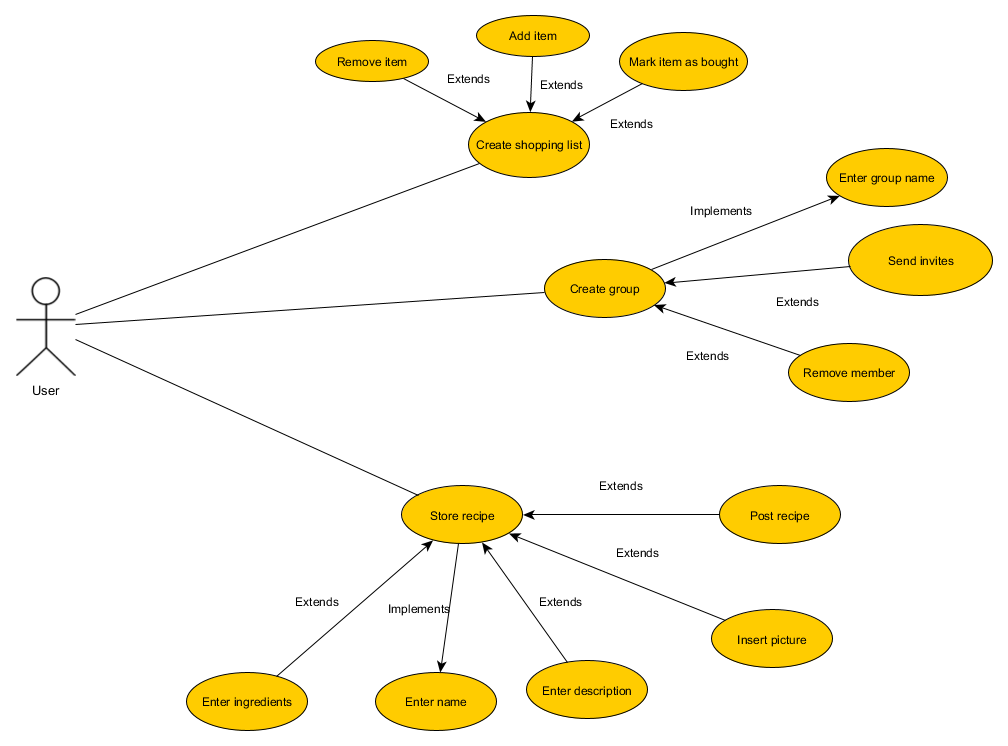
\includegraphics[scale=.5]{UseCase.png}

\subsection{Use Case Details}

\subsubsection{Characteristic Information}

\begin{tabular}{|l|l|}
\hline
Superior business process &  \\ \hline
Goal &  \\ \hline
Precondition &  \\ \hline
Postcondition &  \\ \hline
Involved User &  \\ \hline
Triggering Event &  \\ \hline
\end{tabular}

\subsubsection{GUI to call the use case}

\begin{tabular}{|l|l|}
\hline
Input field & Valid inputs \\ \hline
 &  \\ \hline
\end{tabular}

\subsubsection{Scenario for the standard use}

\begin{tabular}{|l|l|l|}
\hline
Step & User & Activity \\ \hline
 & & \\ \hline
\end{tabular}

\subsubsection{GUIs for the standard use}
\begin{tabular}{|l|l|}
\hline
Input field & Valid inputs \\ \hline
 &  \\ \hline
\end{tabular}
\subsubsection{Scenarios for non-standard uses}

\begin{tabular}{|l|l|l|}
\hline
Step & User & Activity \\ \hline
 & & \\ \hline
\end{tabular}

\subsubsection{GUIs for the non-standard uses}

\begin{tabular}{|l|l|}
\hline
Input field & Valid inputs \\ \hline
 &  \\ \hline
\end{tabular}

\subsubsection{Workflow}

\subsubsection{Open Points}

\pagebreak

\section{Non-functional Requirements}

\pagebreak

\section{Quantity Structure}

\pagebreak

\section{System Architecture and Interfaces}

\pagebreak

\section{Acceptance Criteria}

\pagebreak

\section{Acceptance Criteria}

\pagebreak

\section{References}

\pagebreak

\section{List of Figures}

\pagebreak

\end{document}  